\chapter{11 октября}

\section{Гипотезы}

\begin{definition}
    \textbf{Гипотезой} \(H\) называется предположение о свойствах случайной величины.
\end{definition}

\begin{definition}
    Гипотеза называется \textbf{простой}, если она однозначно определяет распределение, т.е. \(H : \mathcal{F} = \mathcal{F}_1\), где \(\mathcal{F}_1\) --- распределение известного типа с известными параметрами.
\end{definition}

\begin{definition}
    Все остальные гипотезы называются \textbf{сложными}, т.к. они являются объединением конечного или бесконечного числа простых гипотез.
\end{definition}

\begin{definition}[основная модель гипотез]
    Гипотеза \(H_1 = \overline{H_0}\) --- конкурирующая \textit{(альтернативная)} гипотеза, состоящая в том, что основная гипотеза \(H_0\) неверна.
\end{definition}

\begin{remark}
    С помощью статистических методов нельзя \underline{доказать} гипотезу, можно только сказать, что она верна с некоторой уверенностью.
\end{remark}

Основная гипотеза \(H_0\) принимается или отклоняется с помощью \underline{статистики критерия} \(K\):
\[K(X_0 \dots X_n) \to \R = S \cup\!\footnote{Объединение на самом деле дизъюнктно.} \overline{S} \to (H_0, H_1)\]
\[\begin{cases}
        H_0, & \text{если } K \in \overline{S} \\
        H_1, & \text{если } K \in S
    \end{cases}\]

\begin{definition}
    Если точка находится на границе областей \(S\) и \(\overline{S}\), она называется \textbf{критической}.
\end{definition}

\begin{definition}
    \textbf{Ошибка I рода} состоит в том, что нулевая гипотеза отвергается, когда она верна.
\end{definition}

\begin{definition}
    \textbf{Ошибка II рода} состоит в том, что отвергается альтернативная, когда она верна.
\end{definition}

\begin{definition}
    \(\alpha\) --- вероятность ошибки II рода, \(\beta\) --- вероятность ошибки I рода/
\end{definition}

\begin{example}
    \(H_0\) --- деталь годная, \(H_1\) --- деталь бракованная.

    Ошибка I рода --- признать годную деталь бракованной.

    Ошибка II рода --- признать бракованную деталь годной.
\end{example}

\begin{remark}
    При росте выборки вероятности ошибок уменьшаются, при уменьшении вероятности одной ошибки другая вероятность увеличивается.
\end{remark}

\subsection{Способы сравнения критериев}

Пусть имеются критерии \(K_1\) и \(K_2, \alpha_1, \beta_1, \alpha_2, \beta_2\) --- вероятности ошибок при соответствующих критериях, \(h_1\) --- потери в результате ошибке I рода, \(h_2\) --- потери в результате ошибки II рода.

Тогда рассмотрим способы сравнения критериев:
\begin{enumerate}
    \item Минимакс: \(K_1\) не хуже, чем \(K_2\), если \(\max(\alpha_1 h_1, \beta_1 h_2) \leq \max(\alpha_2 h_1, \beta_2 h_2)\)
    \item Критерий называется \textbf{баесовским}, если \(U = \alpha k_1 + \beta k_2\) минимально.
    \item Пусть \(\varepsilon\) --- допустимый уровень ошибки I рода. Обозначим \(K_\varepsilon \coloneqq \{K_i \mid \alpha_i \leq \varepsilon\}\).

          \begin{definition}
              Критерий \(K \in K_\varepsilon\) называется \textbf{наиболее мощным} критерием уровня \(\varepsilon\), если \(\beta \leq \beta_i \ \ \forall i\).
          \end{definition}
\end{enumerate}

\subsection{Критерий согласия}

\begin{definition}
    Критерий \(K\) называется \textbf{критерием асимптотического уровня \(\varepsilon\)}, если вероятность ошибки первого рода \(\alpha\) стремится к \(\varepsilon\) при \(n \to \infty\).
\end{definition}

\begin{definition}
    Критерий \(K\) для проверки гипотезы \(H_0\) против альтернативы \(H_1 = \overline{H_0}\) называется \textbf{состоятельным}, если вероятность ошибки II рода \(\beta \to 0\) при \(n \to \infty\).
\end{definition}

\begin{definition}
    Критерием \textbf{согласия} уровня \(\varepsilon\) называются состоятельные критерии асимптотического уровня \(\varepsilon\).
\end{definition}

\subsection{Построение критериев согласия}

В качестве критериев согласия берётся статистика \(K(X_1 \dots X_n)\) со свойствами:
\begin{enumerate}
    \item Если \(H_0\) верна, то \(K(X_1 \dots X_n) \rightrightarrows Z\) --- известное распределение с известными параметрами.
    \item Если \(H_0\) не верна, то \(K(X_1 \dots X_n) \xrightarrow{P} \infty\)
\end{enumerate}
Для заданного уровня значимость \(\varepsilon\) находим константу \(t_k\), такую что \(P(|Z| \geq t_k) = \alpha\). В результате получаем критерий согласия уровня значимости \(\alpha = \varepsilon\):
\[\begin{cases}
        H_0, & |K| < t_k    \\
        H_1, & |K| \geq t_k
    \end{cases}\]
\begin{theorem}
    Этот критерий является критерием согласия.
\end{theorem}
\begin{proof}\itemfix
    \begin{enumerate}
        \item \(K\) --- критерий асимптотического уровня:

              Пусть \(H_0\) верна. Тогда по построению \(K \rightrightarrows Z\), т.е. \(F_K(x) \to F_Z(x)\) и
              \begin{align*}
                  \alpha & = P(|K| \geq t_k \mid H_0)                                \\
                         & = 1 - P(|K| < t_k)                                        \\
                         & = 1 - (F_K(t_k) - F_K( -t_k))                             \\
                         & \xrightarrow[n \to \infty ]{} 1 - (F_Z(t_k) - F_Z( -t_k)) \\
                         & = P(|Z| \geq t_k)                                         \\
                         & = \varepsilon
              \end{align*}
        \item \(K\) --- состоятельный критерий:

              Пусть \(H_1\) верна. Тогда \(K(X_1 \dots X_n) \xrightarrow[]{P} \infty\), т.е.
              \[\forall C \ \ P(|K| \geq C \mid H_1) \xrightarrow[n \to \infty ]{P} 1 \Rightarrow \beta = P(|K| < t_k \mid H_1) \xrightarrow[n \to \infty ]{P} 0\]
    \end{enumerate}
\end{proof}

\begin{exercise*}
    Гипотеза о среднем нормальной совокупности с известной дисперсией.

    Пусть имеется выборка \((X_1 \dots X_n) \in X \in N(a, \sigma^2)\), причём второй параметр известен.\footnote{Например, мы измеряем что-то инструментом заданной точности.}

    \(H_0: a = a_0, H_1 : a \neq a_0\).

    В качестве статистики критерия возьмём \(\sqrt{n} \cdot \frac{ \overline{X} - a_0}{\sigma}\). Проверим, что оно имеет требуемые свойства:
    \begin{enumerate}
        \item Если \(H_0\) верна, т.е. \(a = a_0\), то \(\sqrt{n} \frac{ \overline{X} - a_0}{\sigma} = \sqrt{n} \frac{ \overline{X} - a}{\sigma} \in N(0, 1)\)
        \item Если \(H_0\) неверно, т.е. \(a \neq a_0\), то \(|K| \to \infty \):

              \[|K| = \left|\sqrt{n} \frac{ \overline{X} - a_0}{\sigma}\right|= \underbrace{\sqrt{n}}_{ \to \infty } \left|\underbrace{\frac{ \overline{X} - a}{\sigma}}_{\in N(0, 1)} + \underbrace{\frac{a - a_0}{\sigma}}_{\neq 0}\right| \xrightarrow[n \to \infty ]{P} \infty\]
    \end{enumerate}

    Таким образом, этот критерий --- критерий согласия. Для уровня значимости \(\alpha = \varepsilon\) выберем \(C\), такую что \(\varepsilon = P(|K| \geq C) \Rightarrow P(|K| < C) = 1 - \varepsilon \Rightarrow 2 \Phi(C) = 1 - \varepsilon \Rightarrow 2 \Phi(C) = \frac{1 - \varepsilon}{2}\)

    Итого:
    \[\begin{cases}
            H_0, & |K| = \left|\sqrt{n} \frac{ \overline{X} - a_0}{\sigma}\right| < C    \\
            H_1, & |K| = \left|\sqrt{n} \frac{ \overline{X} - a_0}{\sigma}\right| \geq C
        \end{cases}\]
    Заметим, что если мы решим это неравенство, то получим доверительный интервал для параметра \(a\) нормального распределения при известном \(\sigma\).
\end{exercise*}

\begin{remark}
    Аналогично можно проверять для неизвестного \(\sigma\), тогда в критерии \(\sigma\) заменится на \(S\).
\end{remark}

\subsection{Доверительные интервалы как критерии гипотез о параметрах распределения}

Пусть имеется выборка \((X_1 \dots X_n)\) случайной величины \(X \in \mathcal{F}_\theta\), где \(\mathcal{F}_\theta\) --- распределение известного типа с неизвестным параметром \(\theta\). Проверяется гипотеза: \(H_0 : \theta = \theta_0\) против \(H_1 : \theta \neq \theta_0\). Пусть для \(\theta\) построен доверительный интервал \((\theta^- , \theta^+)\) надежности \(\gamma\). Тогда следующий критерий является критерием согласия уровня \(\alpha = 1 - \gamma\):
\[\begin{cases}
        H_0, & \theta_0 \in (\theta^- , \theta^+)    \\
        H_1, & \theta_0 \notin (\theta^- , \theta^+)
    \end{cases}\]
\begin{proof}
    \[\alpha = P(\theta_0 \notin (\theta^- , \theta^+) \mid X \in \mathcal{F}_\theta) = 1 - P(\theta_0 \in (\theta^- , \theta^+) \mid X \in \mathcal{F}_\theta) = 1 - \gamma = \alpha\]

    Доказывать состоятельность критерия нужно в каждом случае отдельно.
\end{proof}

\begin{example}
    По выборке объема \(n = 36\) из нормальной совокупности с известным \(\sigma = 1.44\) найдено выборочное среднее \(\overline{X} = 21.36\). Проверить гипотезу \(H_0 : a = 21\) против \(H_1 : a \neq 21\) при уровне значимости \(\alpha = 0.05\).
    \[K = \sqrt{n} \frac{ \overline{X} - a_0}{\sigma} = \sqrt{36} \frac{21.6 - 21}{1.44} = 2.5\]
    \[\Phi(t_k) = \frac{1 - \alpha}{2} = 0.475\]
    \[t_k = 1.96\]
    Т.к. \(|K| = 2.5 > 1.96\), гипотеза отклоняется.
\end{example}

В математических пакетах могут не сравнивать с критической точкой, а считать статистику и искать вероятность.

\begin{remark}
    Следующий материал был рассказан на практике 13 октября.
\end{remark}

\subsection{Распределение Коши}

Пусть дан источник некоторого излучения в точке \((0, 1)\), который равномерно посылает лучи во все стороны.

Случайная величина \(\xi\) --- точка пересечения луча с осью \(OX\).

Найти \(F_\xi(x), f_\xi(x), \E \xi\).

\begin{figure}[h]
    \centering
    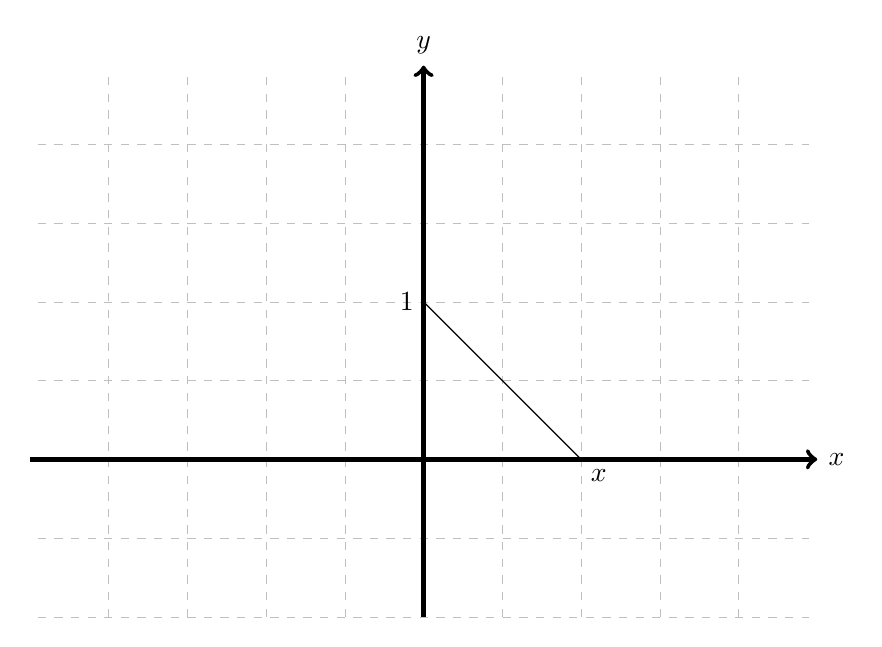
\begin{tikzpicture}
        \draw[help lines, color=gray!50, dashed] (-4.9,-2) grid (4.9,4.9);
        \draw[->,ultra thick] (-5,0)--(5,0) node[right]{$x$};
        \draw[->,ultra thick] (0,-2)--(0,5) node[above]{$y$};
        \draw (0, 2) node[left] {1} -- (2, 0);
        \node[below right] at (2, 0) {\(x\)};
        % \draw (0, 2) arc (180:360:0.1);
    \end{tikzpicture}
    \caption{Источник}
\end{figure}

\[F_\xi(x) = P(\xi < x) = P(\xi < 0) + P(0 < \xi < x) = 0.5 + \frac{1}{\pi} \arctg x\]
\[f_\xi(x) = F_\xi'(x) = \frac{1}{\pi} \frac{1}{x^2 + 1}\]
\[\E \xi = \int_{ - \infty }^{ + \infty } x f_\xi(x) = \int_{ - \infty }^{ + \infty } x \frac{1}{\pi} \frac{1}{x^2 + 1} dx = \frac{1}{2 \pi} \ln(1 + x^2) \Big|_{ - \infty }^{ + \infty}, \nexists\]

Пусть теперь источник сдвинут на \(\theta\) по оси \(x\). Тогда \(f_\xi(x) = \frac{1}{\pi (1 + (x - \theta)^2)}\). Попробуем оценить \(\theta\). \(\overline{X}\) не работает, т.к. оно убежит на бесконечность: \(\E \frac{S_n}{n} = \E X\). Оценим с помощью медианы. По симметрии \(\theta = \mathrm{Me} \xi\).

\[\mathrm{Me}^* = \begin{cases}
        X_{(k + 1)},                     & n = 2k + 1 \\
        \frac{X_{(k)} + X_{(k + 1)}}{2}, & n = 2k
    \end{cases}\]

\begin{theorem}
    Если \(f(\mathrm{Me}) \neq 0\), то \(\mathrm{Me}^* \xrightarrow{P} \mathrm{Me}\), причём сходится со скоростью \(\frac{1}{\sqrt{n}}\).
\end{theorem}

В целом при большом числе выбросов медиана помогает. Например, оценивать зарплату нужно по медиане, а не по среднему.

У медианы также есть свои недостатки: она сходится медленнее, чем выборочное среднее --- эффективность обычно ниже на 20-30\%, но бывают и случаи хуже.

Есть и другие оценки, например \textbf{усечённое среднее}. Выкидываются наименьшие и наибольшие \(k\) точек и считается выборочное среднее:
\[\frac{\sum\limits_{i= k + 1}^{n - k} X_{(i)}}{n - 2k}\]
Несложно заметить, что это нечто промежуточное между выборочным средним и медианой --- если \(k = 0\), то получаем выборочное среднее, если \(k = \frac{n - 1}{2}\), то получаем медиану.

Другой пример: составим по исходной выборке выборку объема \(\frac{n(n - 1)}{2}\), состоящую из \(\frac{X_i + X_j}{2}, 1 \leq i,j \leq n\). \textbf{Среднее Уолша} --- медиана этой выборки. У этой оценки эффективность падает на \(\approx 12\%\) относительно выборочного среднего.

\begin{exercise}
    Дано \(n\) призывников с вероятностью болезни \(p = 0.01\). Разбиваем призывников на группы по \(k\) человек в группе. Считаем, что \(n \divided k\), т.е. групп \(\frac{n}{k}\). В каждой группе:
    \begin{itemize}
        \item Если суммарный результат отрицательный, то \(1\) анализ.
        \item Иначе \(k + 1\) анализ.
    \end{itemize}

    Найти оптимиальное значение \(k\) и среднее значение числа анализов.
\end{exercise}
\begin{solution}
    \(\xi_i\) --- число анализов в \(i\)-той группе.

    \[P(\xi_i = 1) = (1 - p)^k \quad P(\xi_i = k + 1) = 1 - (1 - p)^k\]
    \[\E \xi_i = (1 - p)^k + (k + 1)(1 - (1 - p)^k) = k + 1 - k(1 - p)^k\]
    \[\xi = \frac{n}{k} \cdot \xi_i\]
    \[\E \xi = n\left(1 + \frac{1}{k} - (1 - p)^k\right) = f(k)\]
    Т.к. \(p\) мало, пусть оно \(p \to 0\). \((1 - p)^k \sim 1 - pk\).
    \[f(k) \sim n \left(\frac{1}{k} + pk\right)\]
    \[f'(k) = n \left( - \frac{1}{k^2} + p \right) = 0\]
    \[k = \frac{1}{\sqrt{p}} = 10\]
    \[\E \xi \approx n \left(\frac{1}{10} + 0.01 \cdot 10\right) = 0.2 n\]
\end{solution}
